\documentclass[SDSUThesis.tex]{subfiles} 
\begin{document}

\newpage

%% numbers following sections with A, B, C..
\appendix
\label{appendix}
\begin{center}
APPENDIX\\
\end{center}
\addcontentsline{toc}{section}{APPENDIX}

\section{DETAILED STEPS OF THE SDLC}
\label{app:detailedSDLC}

    The SDLC often contains more than the five basic steps of requirements, design,
    implementation, testing, and  deployment/maintenance.  Those are the high-level
    phases, but many steps are required to complete each phase.  The following list
    provides a more detailed list of what needs to be accomplished in the 
    entire life cycle of software development. These steps do not need 
    to occur in a sequential fashion.

    \begin{easylist}[itemize]
        & Identify the Work/Task/Project
        && Get Initial Idea 
        && Obtain Details
        & Estimate
        && Create an Estimate (What is included? What is the output? days/dollars/hours/reqs)
        && Obtain Approval 
        && Quit or Go Forward
        & Document Requirements
        && Identify the Requirements
        && Detail the Requirements
        & Design The Software
        && Find System Integrations
        && Identify Functional Specs
        && Detail the Functional Specs
        & Development of all the tasks in Design and Requirements
        && Identify the Coding Tasks
        && Write the Code/Develop the solution
        && Write the Unit Tests
        & Test
        && Create Test Plans and Cases
        && Run Test Plans and Cases
        & Deployment
        && Create Deployment Steps
        && Run Deployment Steps
        & Maintenance
        && Capture Bugs
        && Survey Users
        & Start Again
    \end{easylist}

\section{SDLC-AE SOURCE CODE}

%% set appendix to single space for the source code
\linespread{1.0}

%% options for lists
\lstset{ %
  basicstyle=\small,        % the size of the fonts that are used for the code
  breakatwhitespace=false,         % sets if automatic breaks should only happen at whitespace
  breaklines=true,                 % sets automatic line breaking
  commentstyle=\color{ForestGreen},    % comment style
  frame=single,                    % adds a frame around the code
  keepspaces=true,                 % keeps spaces in text, useful for keeping indentation of code (possibly needs columns=flexible)
  keywordstyle=\color{blue},       % keyword style
  numbers=left,                    % where to put the line-numbers; possible values are (none, left, right)
  numbersep=5pt,                   % how far the line-numbers are from the code
  numberstyle=\tiny\color{gray}, % the style that is used for the line-numbers
  rulecolor=\color{black},         % if not set, the frame-color may be changed on line-breaks within not-black text (e.g. comments (green here))
  showspaces=false,                % show spaces everywhere adding particular underscores; it overrides 'showstringspaces'
  showstringspaces=false,          % underline spaces within strings only
  showtabs=false,                  % show tabs within strings adding particular underscores
  stepnumber=1,                    % the step between two line-numbers. If it's 1, each line will be numbered
  tabsize=4,                       % sets default tabsize to 2 spaces
}

\subsection{SQL CODE - DATA TABLES}
    \lstinputlisting[language=SQL, label=src:rawSQL]{source/raw_tables.sql}

\subsection{SQL CODE - SCORE TABLES}
    \lstinputlisting[language=SQL, label=src:scoreSQL]{source/score_tables.sql}
    
\subsection{SQL CODE - FINAL SCORE TABLES}
    \lstinputlisting[language=SQL, label=src:overallscoreSQL]{source/overall_score_tables.sql}
    

\section{CASE STUDY SOURCE CODE} 
\label{app:case}
    A full set of the source code and applicable output is available 
    at \cite{Swanstrom2015s}.


    \subsection{QUALITY HISTORICAL R CODE AND ANALYSIS}
    \label{app:quality-history}
        \lstinputlisting[language=R]{source/quality_historical.R}
        The source code for the selected baseline quality function
        can be seen above. The output for the linear model can be seen below.
        \lstinputlisting{source/quality_output.txt}
        
        Some diagnostic plots for the baseline quality function
        can be seen in Figure \ref{fig:quality-diag}.  The normal probability plot,
        a.k.a. Q-Q Plot, shows the errors are not exactly normally distributed, but
        the baseline quality function had good predictive power as shown by the
        high $R^2$. The fitted versus
        residuals plot indicates a lack of heteroscedasticity.  
        \begin{figure}[ht]
            \centering
            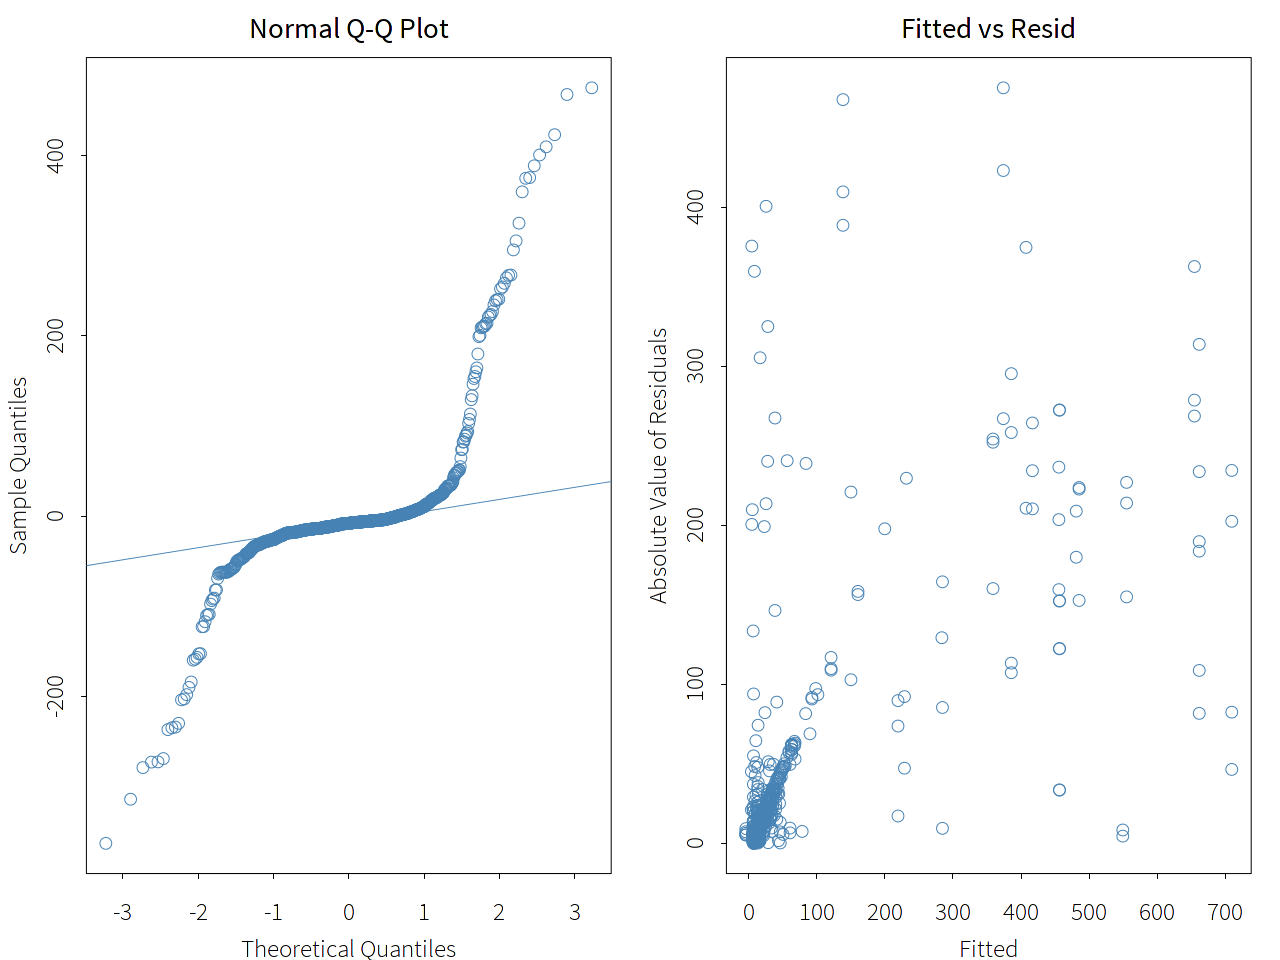
\includegraphics[scale=.25]{images/quality_diag.png}
            \caption{QUALITY DIAGNOSTIC PLOTS}
            \label{fig:quality-diag}
        \end{figure}
        
        Figure \ref{fig:quality-pairs} shows the presence of some
        possible multicolinearity.  As a result, ridge regression
        was used to create a model, but the results were very similar
        to the original baseline quality function. Therefore,
        ridge regression was not chosen. 
        \begin{figure}[ht]
            \centering
            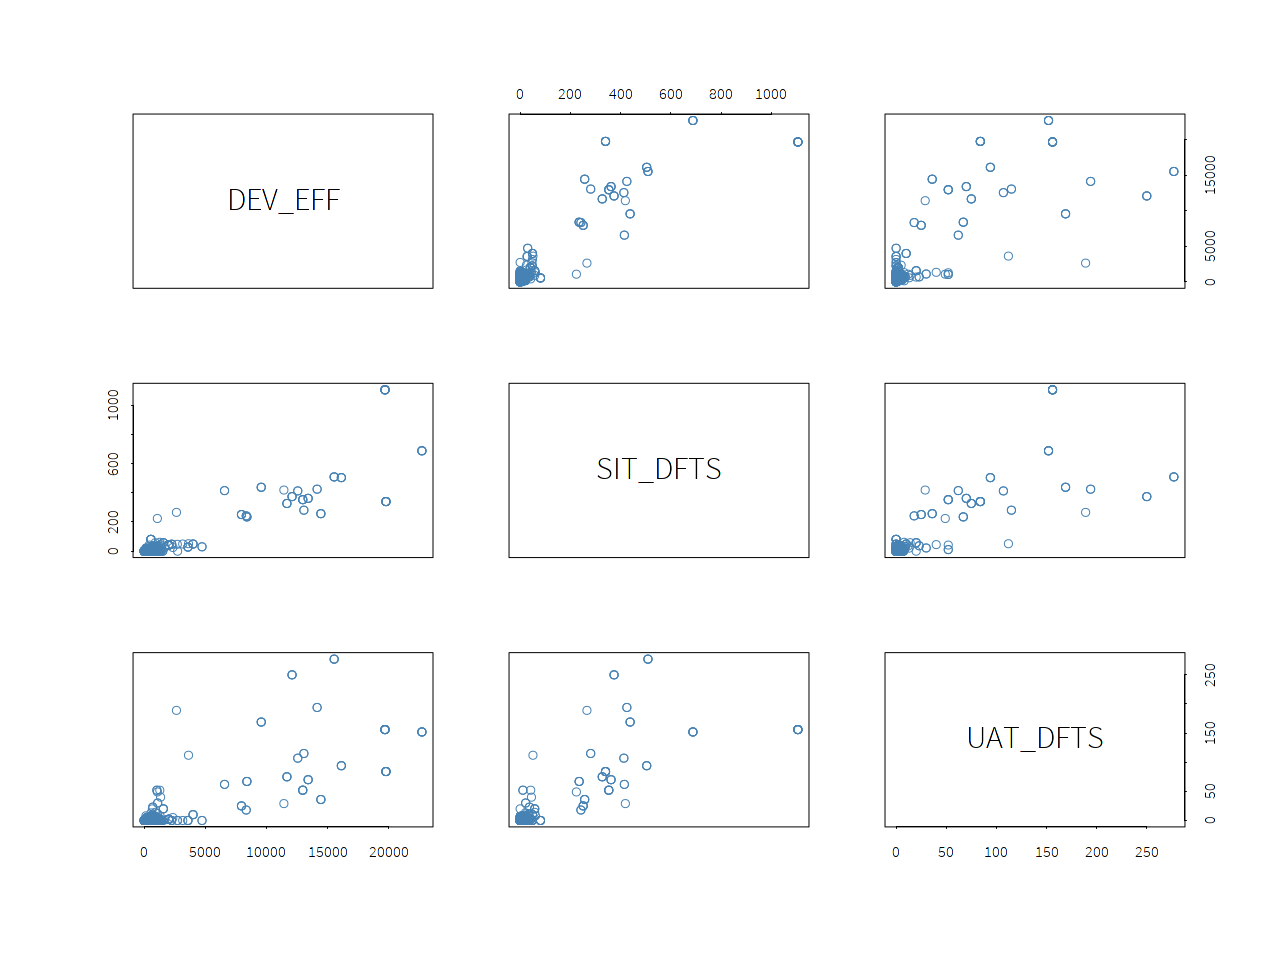
\includegraphics[scale=.3]{images/quality_pairs.png}
            \caption{QUALITY PAIRS PLOT OF INDEPENDENT VARIABLES}
            \label{fig:quality-pairs}
        \end{figure}
        
    \subsection{BAR CHART - R CODE}
        This is a code for generating a bar chart.  It is used for reporting
        the scores of all the elements.
        \lstinputlisting[language=R, label=src:barchart]{source/barchart.R}
        
    \subsection{QUALITY SCORES - R CODE}
        \lstinputlisting[language=R, label=src:quality]{source/quality.R}
        
    \subsection{AVAILABILITY SCORES - R CODE}
        \lstinputlisting[language=R, label=src:availability]{source/availability.R}
        
    \subsection{SCHEDULE SCORES - R CODE}
        \lstinputlisting[language=R, label=src:schedule]{source/schedule.R}
        
    \subsection{REQUIREMENTS SCORES - R CODE}
        \subsubsection{REQUIREMENTS HISTOGRAM}
        \label{app:requirements-hist}
            Figure \ref{fig:req-hist} shows a histogram of the data
            for requirements.  The histogram is based upon the
            fraction, $\frac{Scheduled Requirements}{Actual Requirements}$. The
            values where the fraction equals one have been left out of the histogram.
            So, the histogram show only the data that did not deliver exactly
            on the number of requirements. Rarely are more requirements actually 
            delivered than what was scheduled.  On the opposite side, the histogram
            bars shrink as they approach zero indicating that it is more common
            to miss a few requirements than all the requirements.
            
            \begin{figure}[ht]
                \centering
                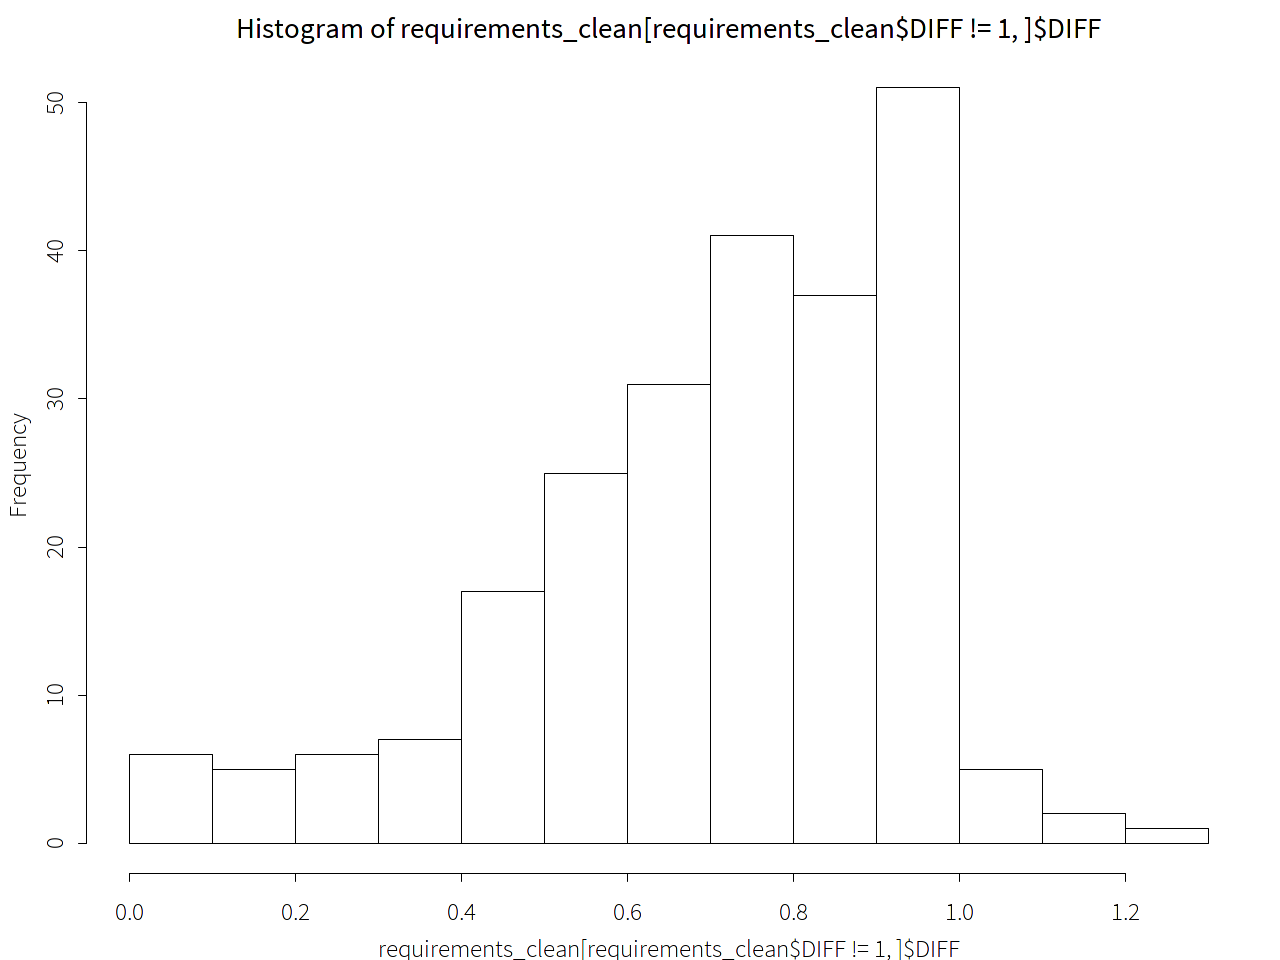
\includegraphics[scale=.3]{images/req_hist.png}
                \caption{REQUIREMENTS DATA HISTOGRAM (ACTUAL/SCHEDULED)}
                \label{fig:req-hist}
            \end{figure}
        
        \subsubsection{REQUIREMENTS R CODE}
        \lstinputlisting[language=R, label=src:requirements]{source/requirements.R}
        
        
    \subsection{OVERALL SCORES - R CODE}
        \lstinputlisting[language=R, label=src:overall]{source/overall.R}
        
    


\section{ADDITIONAL SDLC DATA NEEDS}

    This appendix describes some additional SDLC attributes that could be tracked to help improve
    estimation.  The SDLC-AE could be expanded to include the following.

    \subsection{ESTIMATION}
    
        The following are additional data points that could be tracked for project estimation.
        \begin{easylist}[itemize]
            & Change to database structure  
            & Modify database data    
            & Create a new database, number of new databases  
            & Server configuration changes required   
            & New servers required   
            & Number of people involved  
            & Number of (sub)systems involved  
            & Estimation date
            & Number of days allowed
            & List of other attributes
            & Number of screens involved 
            & Actual values (hours, days, dollars) 
            & Estimated values
            && Estimated development hours: 
                The number of development hours estimated for a 
                project, this is just developer hours
            && Estimated documentation hours: 
                The number of documentation hours estimated for a project
            && Estimated testing hours:
                The number of testing hours estimated for a project
            && Estimated deployment hours: 
                The number of estimated hours required to 
                deploy the project
        \end{easylist}
    
    \subsection{REQUIREMENTS}
    
        The following are additional data points that could be tracked for the requirements phase of an
        SDLC project.
        \begin{easylist}[itemize]
            & Title
            & Description
            & Author
            & Project
            & Date
            & Comments
            &&  Date
            &&  Comment text
            &&  Author
        \end{easylist}
    
    \subsection{DEVELOPMENT}
    
        The following are additional data points that could be tracked for the development phase of an
        SDLC project.
        \begin{easylist}[itemize]
            & Project
            & Release
            & List of files
            & Author
            & Date started
            & Completion date
            & Number of unit tests
            & Lines of code
            & Percentage of automated test coverage
            & Others
        \end{easylist}
    
    
    \subsection{TESTING}
        The following are additional data points that could be tracked during, before, and after the
        testing phase of an SDLC project.
        \begin{easylist}[itemize]
            & Project
            & Release
            & Title
            & description]
            & Author]
            & Date started
            & Date executed
            & Status (pending, pass, fail)
            & Comments 
            && Date
            && Comment text
            && Author
        \end{easylist}
    
    \subsection{IMPLEMENTATION}
    
        The following are additional data points that could be tracked for the implementation of a project.
        \begin{easylist}[itemize]
            & Project
            & Release
            & date Entered
            & Date Scheduled
            & Date Executed
            & Ordering/Prerequisites
            & Comments
            && date
            && Comment text
            && Author
        \end{easylist}
    
    \subsection{MAINTENANCE (DEFECTS)}
    
        The following are additional data points that could be tracked for maintenance of a project.
        \begin{easylist}[itemize]
            & Project
            & Release
            & Description
            & Date Entered
            & Date fixed
            & Comments
            && Date
            && Comment text
            && Author
        \end{easylist}

\end{document}